\documentclass{beamer}
\usepackage{graphicx}
\usepackage{amsmath}    % Necesario para \text y \boxed en las ecuaciones
\usepackage{tabularx}   % Necesario para las tablas ajustables
\usepackage{booktabs}   % Necesario para las líneas profesionales de las tablas
\usepackage{xcolor}     % Para los colores del análisis de datos

\usetheme{Madrid}
\usecolortheme{default}

\title{OnlyQrs}
\subtitle{Detección de enlaces maliciosos mediante análisis de códigos QR}
\author{Felipe Blasquez \and Felipe Cortés}
\institute{Pontificia Universidad Católica de Chile}
\date{\today}

\begin{document}

%------------------------------------------------

\begin{frame}
    \titlepage
\end{frame}

%------------------------------------------------

\begin{frame}{Motivación}
\begin{itemize}
    \item Creciente uso de códigos QR en servicios digitales.
    \item Aparición de ataques de \textbf{Quishing} (QR + Phishing).
    \item Los usuarios no pueden inspeccionar fácilmente el contenido de un QR.
    \item Necesidad de verificar enlaces antes de acceder a ellos.
\end{itemize}
\end{frame}

%------------------------------------------------

\begin{frame}{¿Qué es el Quishing?}
\begin{columns}

\column{0.55\textwidth}
\begin{itemize}
    \item Ataque basado en códigos QR maliciosos.
    \item Redirige a sitios fraudulentos.
    \item Busca robar credenciales o información sensible.
    \item Variante moderna del phishing tradicional.
\end{itemize}

\column{0.45\textwidth}

\vspace{1cm}
\centering
\includegraphics[
    width=\textwidth,
    height=0.75\textheight,
    keepaspectratio
]{img/qishing.png}

\end{columns}
\end{frame}

%------------------------------------------------

\begin{frame}{Objetivo del Proyecto}

\begin{block}{Objetivo}
Diseñar una plataforma capaz de detectar amenazas asociadas a URLs obtenidas desde códigos QR mediante la combinación de múltiples fuentes de inteligencia y análisis heurístico.
\end{block}

\vspace{0.5cm}

Objetivos específicos:

\begin{itemize}
\item Detectar enlaces maliciosos antes de que el usuario los visite.
\item Reducir el riesgo de ataques de phishing y malware.
\item Integrar múltiples motores de inteligencia de amenazas.
\item Traducir resultados técnicos a lenguaje comprensible.
\end{itemize}

\end{frame}

%------------------------------------------------

\begin{frame}{Arquitectura del Sistema}

\centering

% Usamos resizebox para que la cadena no se desborde de la diapositiva
\resizebox{\textwidth}{!}{
$
\boxed{\text{Usuario}}
\rightarrow
\begin{array}{c}
    \boxed{\text{Backend OnlyQRs}} \\
    \downarrow \\
    \boxed{\text{PostgreSQL}}
\end{array}
\rightarrow
\boxed{
    \begin{array}{c}
    \text{Whois} \\
    \text{VirusTotal} \\
    \text{Google Safe Browsing} \\
    \text{URLScan} \\
    \text{URLHaus} \\
    \text{PhishDestroy} \\
    \text{Heurística Propia}
    \end{array}
}
\rightarrow
\boxed{\text{Motor de Scoring}}
\rightarrow
\boxed{\text{Gemini}}
\rightarrow
\boxed{\text{Resultado Final}}
$
}

\vspace{0.6cm}

\begin{itemize}
    \item \textbf{Frontend:} Interfaz de usuario desarrollada en React.
    \item \textbf{Backend (OnlyQRs):} Orquestador central de las peticiones.
    \item \textbf{Base de Datos (PostgreSQL):} Almacenamiento del historial de escaneos vía Sequelize, utilizando \texttt{JSONB} para guardar métricas y telemetría cruda.
    \item \textbf{Capa de Inteligencia:} Consultas en paralelo a múltiples servicios de seguridad y análisis heurístico.
    \item \textbf{Evaluación (IA):} Motor de Scoring integrado con Gemini para emitir el veredicto definitivo.
\end{itemize}

\end{frame}

%------------------------------------------------

\begin{frame}{Flujo de Funcionamiento}

\begin{enumerate}
\item Usuario escanea un QR.
\item Se extrae la URL.
\item Se ejecutan 7 estrategias en paralelo.
\item Se consolidan los resultados.
\item Se calcula un score de riesgo.
\item Gemini genera explicación para el usuario.
\item Se muestra el resultado final.
\end{enumerate}


\end{frame}

%------------------------------------------------
\begin{frame}{Capa de inteligencia: Modelo 6+1}

\begin{table}[htbp]
\centering
\caption{Estrategias de Detección y Objetivos de Análisis del Sistema}
\label{tab:estrategias_deteccion}
\begin{tabularx}{\textwidth}{l X}
\toprule
\textbf{Estrategia} & \textbf{Objetivo} \\
\midrule
Whois & Edad del dominio \\
VirusTotal & Reputación global \\
Google Safe Browsing & Listas negras \\
URLScan & Telemetría histórica \\
URLHaus & Malware activo \\
PhishDestroy & Campañas phishing \\
Heurística propia & Día Cero \\
\bottomrule
\end{tabularx}
\end{table}

\end{frame}

%------------------------------------------------
\begin{frame}{Motor de Heurística Propio}

Evalúa múltiples vectores de riesgo en tiempo real mediante análisis estático:

\vspace{0.2cm}

\begin{columns}[T]
    \begin{column}{0.5\textwidth}
        \textbf{Análisis Estructural}
        \begin{itemize}
            \item Direcciones IP directas.
            \item Exceso de subdominios y guiones.
            \item Puertos de conexión no estándar.
            \item Longitud anómala ($>75$ caracteres).
        \end{itemize}
    \end{column}
    
    \begin{column}{0.5\textwidth}
        \textbf{Detección de Engaño}
        \begin{itemize}
            \item \textit{Brand Spoofing} (bancos, retail).
            \item TLDs de baja reputación (\texttt{.xyz}, \texttt{.top}).
            \item Doble extensión (\texttt{.pdf.exe}).
            \item Ofuscación de credenciales (\texttt{@}).
        \end{itemize}
    \end{column}
\end{columns}

\vspace{0.5cm}

\begin{block}{Objetivo: Protección Día Cero (Zero-Day)}
Calcular un \textit{Risk Score} ponderado para detectar amenazas en el instante en que son creadas, mucho antes de que sean reportadas en listas negras tradicionales.
\end{block}

\end{frame}


%------------------------------------------------
\begin{frame}{Algoritmo de Puntuación}

\[
RiskScore \in [0,100]
\]

Cada estrategia aporta evidencia ponderada.

\vspace{0.5cm}

Clasificación:

\begin{itemize}
\item SAFE (0-20)
\item LOW (21-40)
\item MEDIUM (41-60)
\item HIGH (61-80)
\item CRITICAL (81-100)
\end{itemize}

\end{frame}

%------------------------------------------------
\begin{frame}{Rol de Gemini}

La IA no toma decisiones de seguridad.

\vspace{0.5cm}

\textbf{Backend}
\begin{itemize}
\item Calcula el riesgo.
\item Determina el veredicto.
\end{itemize}

\textbf{Gemini}
\begin{itemize}
\item Interpreta resultados.
\item Genera explicación amigable.
\item Traduce telemetría compleja.
\end{itemize}

\end{frame}

%------------------------------------------------
\begin{frame}{Análisis Histórico y Dashboard Ejecutivo}

\begin{columns}[T] 
    
    % COLUMNA IZQUIERDA: Flujo de procesamiento
    \begin{column}{0.5\textwidth}
        \begin{block}{Pipeline de Análisis (Backend)}
            \begin{enumerate}
                \item \textbf{Extracción (PostgreSQL):} Recuperación de todos los registros históricos de escaneo.
                \item \textbf{Cálculo Estático (Node.js):} Agrupación determinista por nivel de riesgo para \textbf{evitar alucinaciones} numéricas de la IA.
                \item \textbf{Inferencia Semántica (Gemini):} Análisis de patrones sobre una muestra acotada de URLs maliciosas.
                \item \textbf{Consumo (React):} Entrega de resultados para visualización en el dashboard.
            \end{enumerate}
        \end{block}
    \end{column}

    % COLUMNA DERECHA: Características Técnicas
    \begin{column}{0.45\textwidth}
        \vspace{0.2cm}
        \textbf{Características del Motor IA:}
        
        \begin{itemize}
            \item \textbf{JSON Estricto:} Prompt engineering diseñado para forzar a Gemini a devolver una estructura de datos predefinida.
            \item \textbf{Eficiencia de Tokens:} Filtrado inteligente que solo envía métricas pre-calculadas y top 30 amenazas.
            \item \textbf{Resiliencia (Fallback):} Si la API de Google falla o devuelve un JSON corrupto, el sistema genera un reporte estático automático sin romper el frontend.
        \end{itemize}
    \end{column}

\end{columns}

\vspace{0.4cm}

\begin{exampleblock}{Reporte Generado (Estructura)}
    \small
    \textbf{1. Overview:} Estado global de la seguridad.\\
    \textbf{2. Top Threat:} Vectores y marcas más suplantadas.\\
    \textbf{3. Infrastructure:} Patrones en dominios (ej. TLDs sospechosos).\\
    \textbf{4. Recommendation:} Acciones mitigatorias sugeridas.
\end{exampleblock}

\end{frame}

%------------------------------------------------
\begin{frame}{Demostración de la Aplicación: Móvil}

\centering

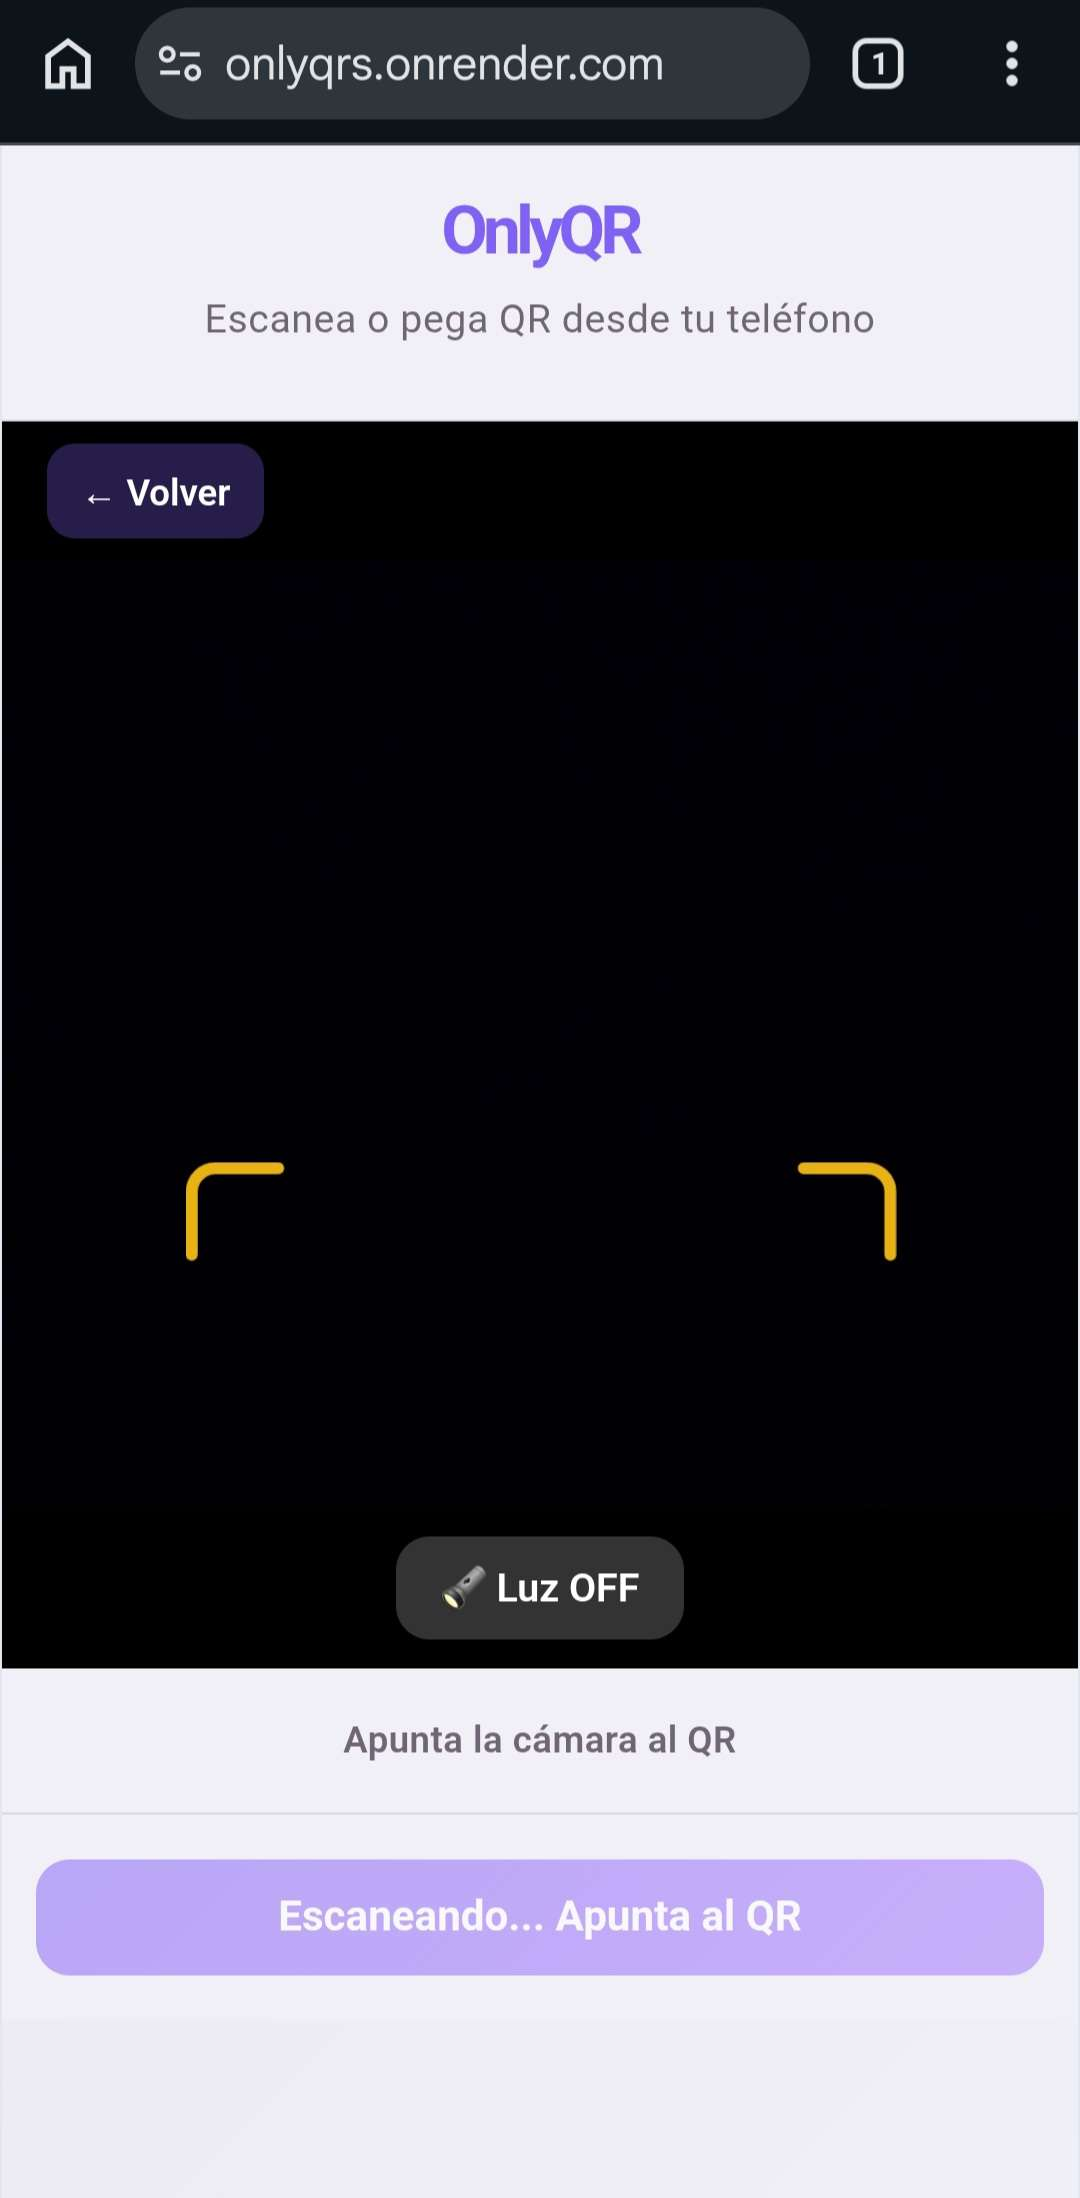
\includegraphics[
    width=\textwidth,
    height=0.75\textheight,
    keepaspectratio
]{img/ss1_movil.jpg}

\end{frame}

%------------------------------------------------

\begin{frame}{Demostración de la Aplicación: Móvil}

\centering

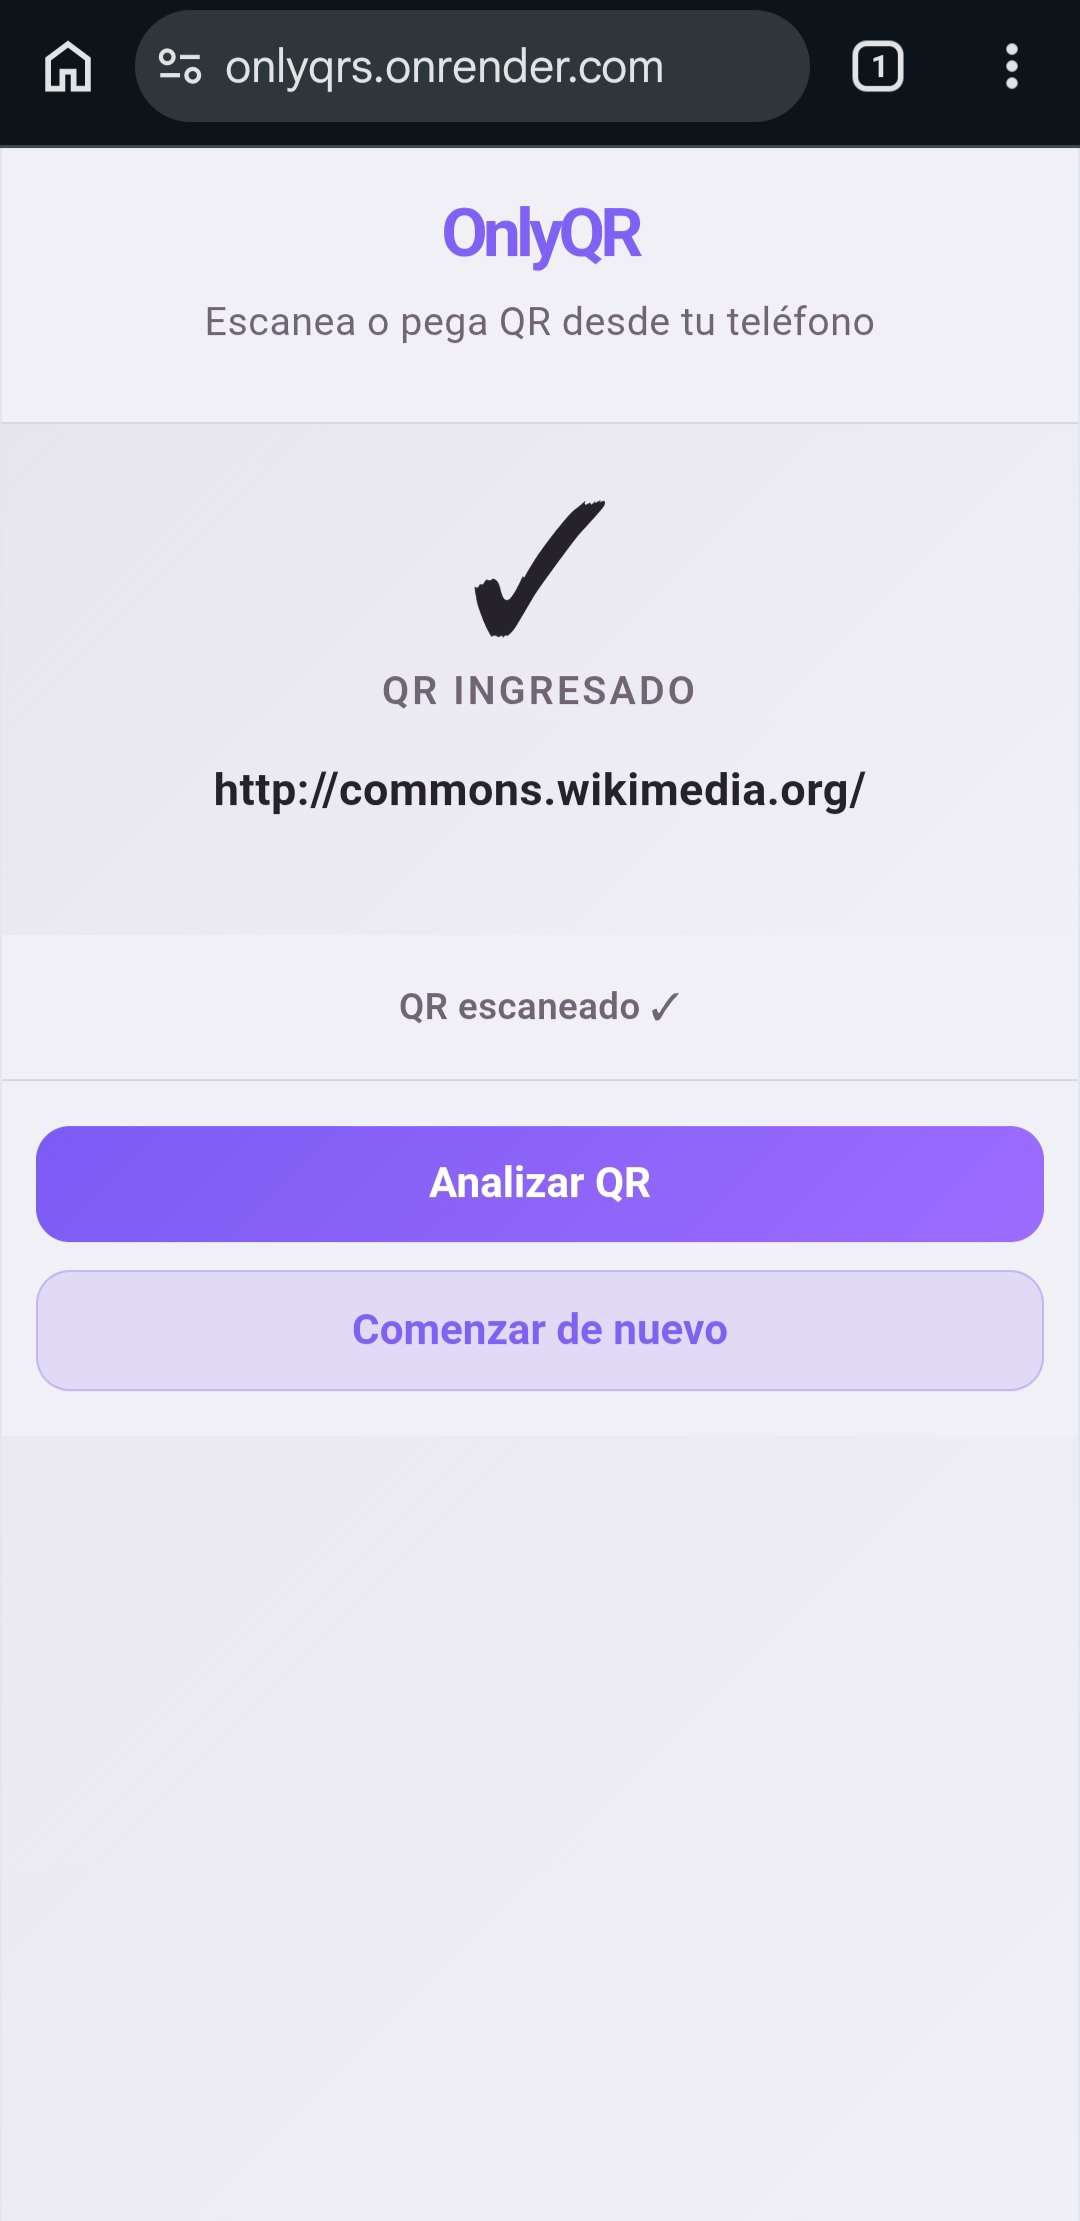
\includegraphics[
    width=\textwidth,
    height=0.75\textheight,
    keepaspectratio
]{img/ss2_movil.jpg}

\end{frame}

%------------------------------------------------

\begin{frame}{Demostración de la Aplicación: Móvil}

\centering

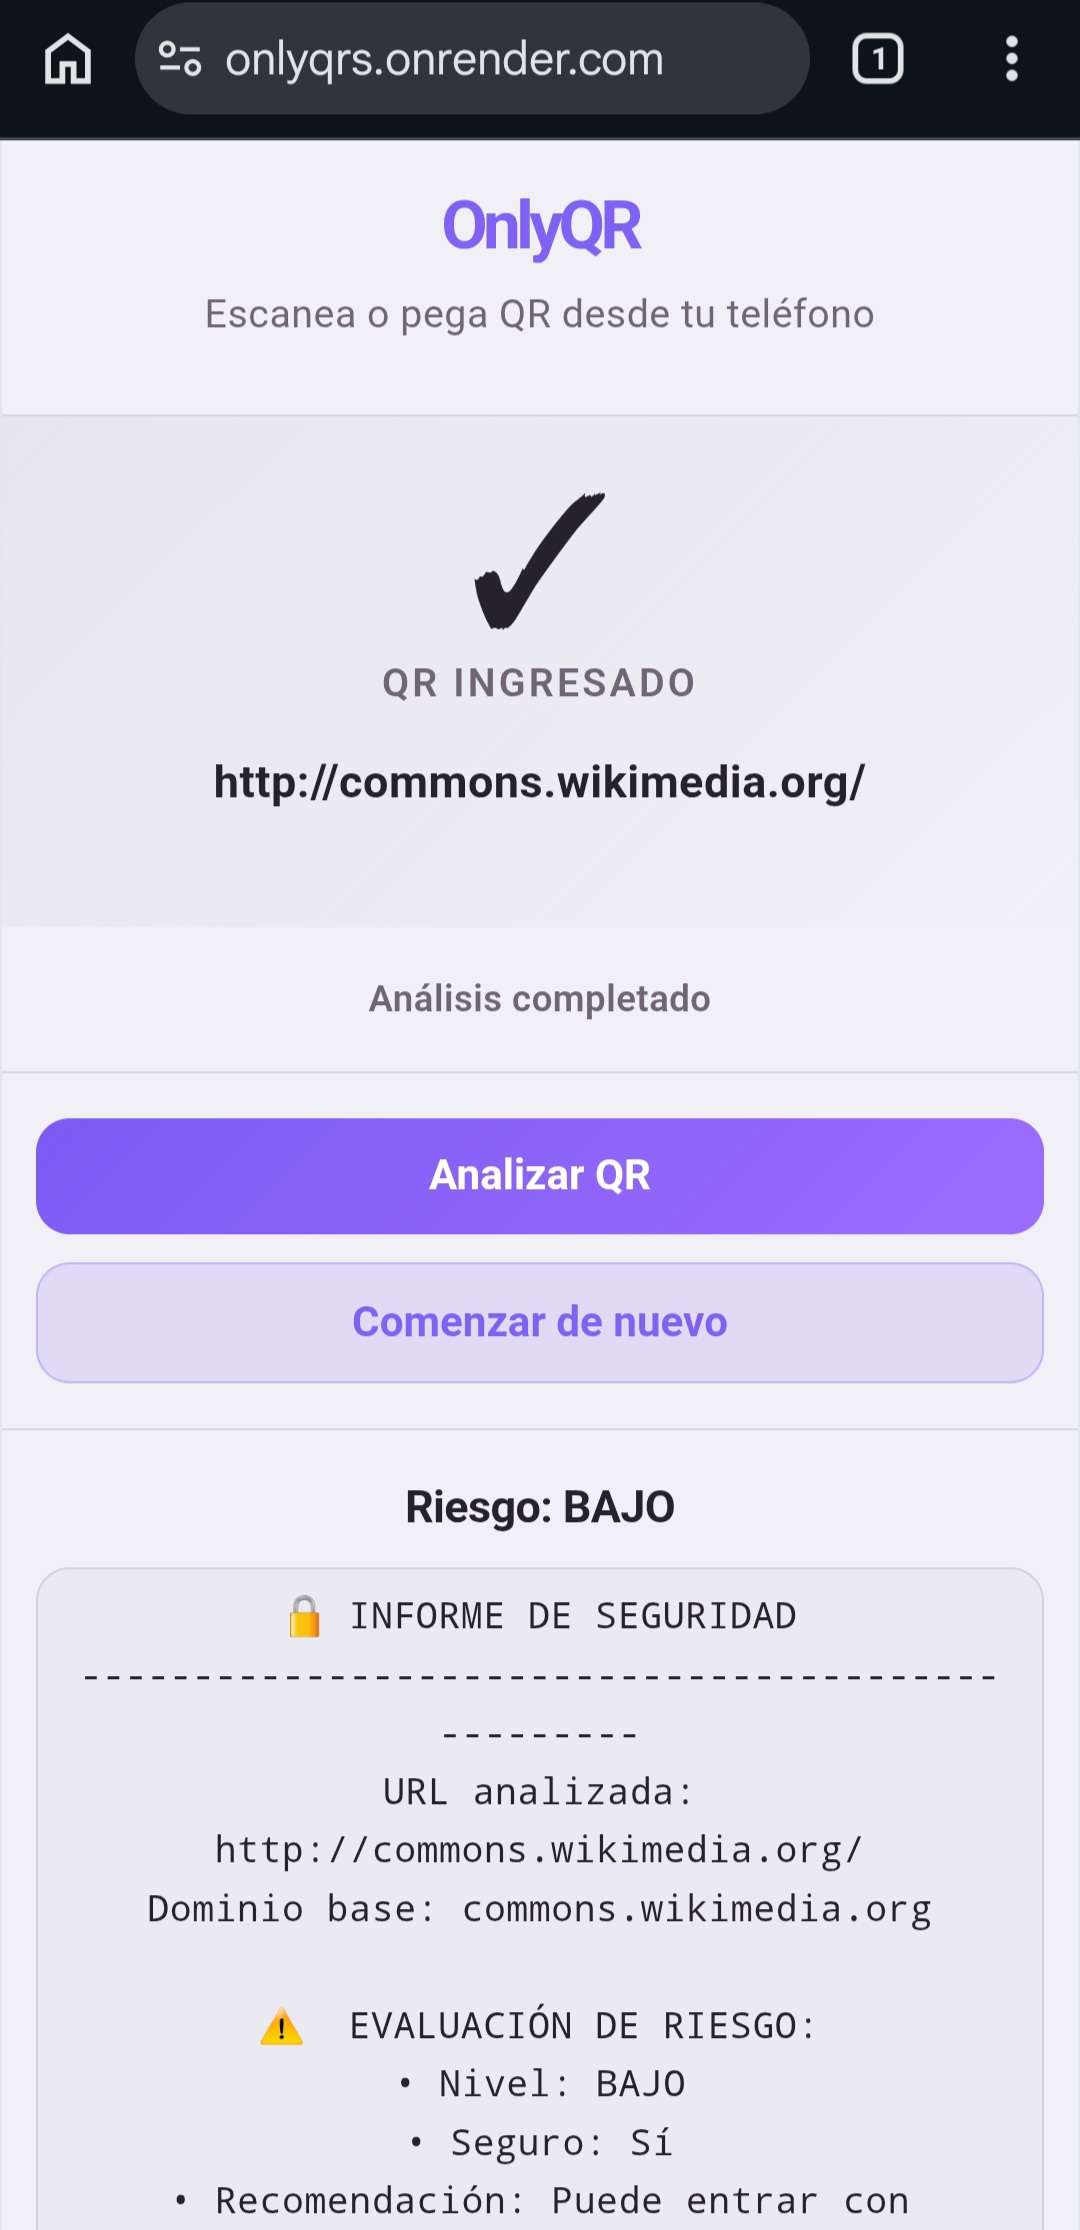
\includegraphics[
    width=\textwidth,
    height=0.75\textheight,
    keepaspectratio
]{img/ss3_movil.jpg}

\end{frame}

%------------------------------------------------

\begin{frame}{Demostración de la Aplicación: Web}

\centering

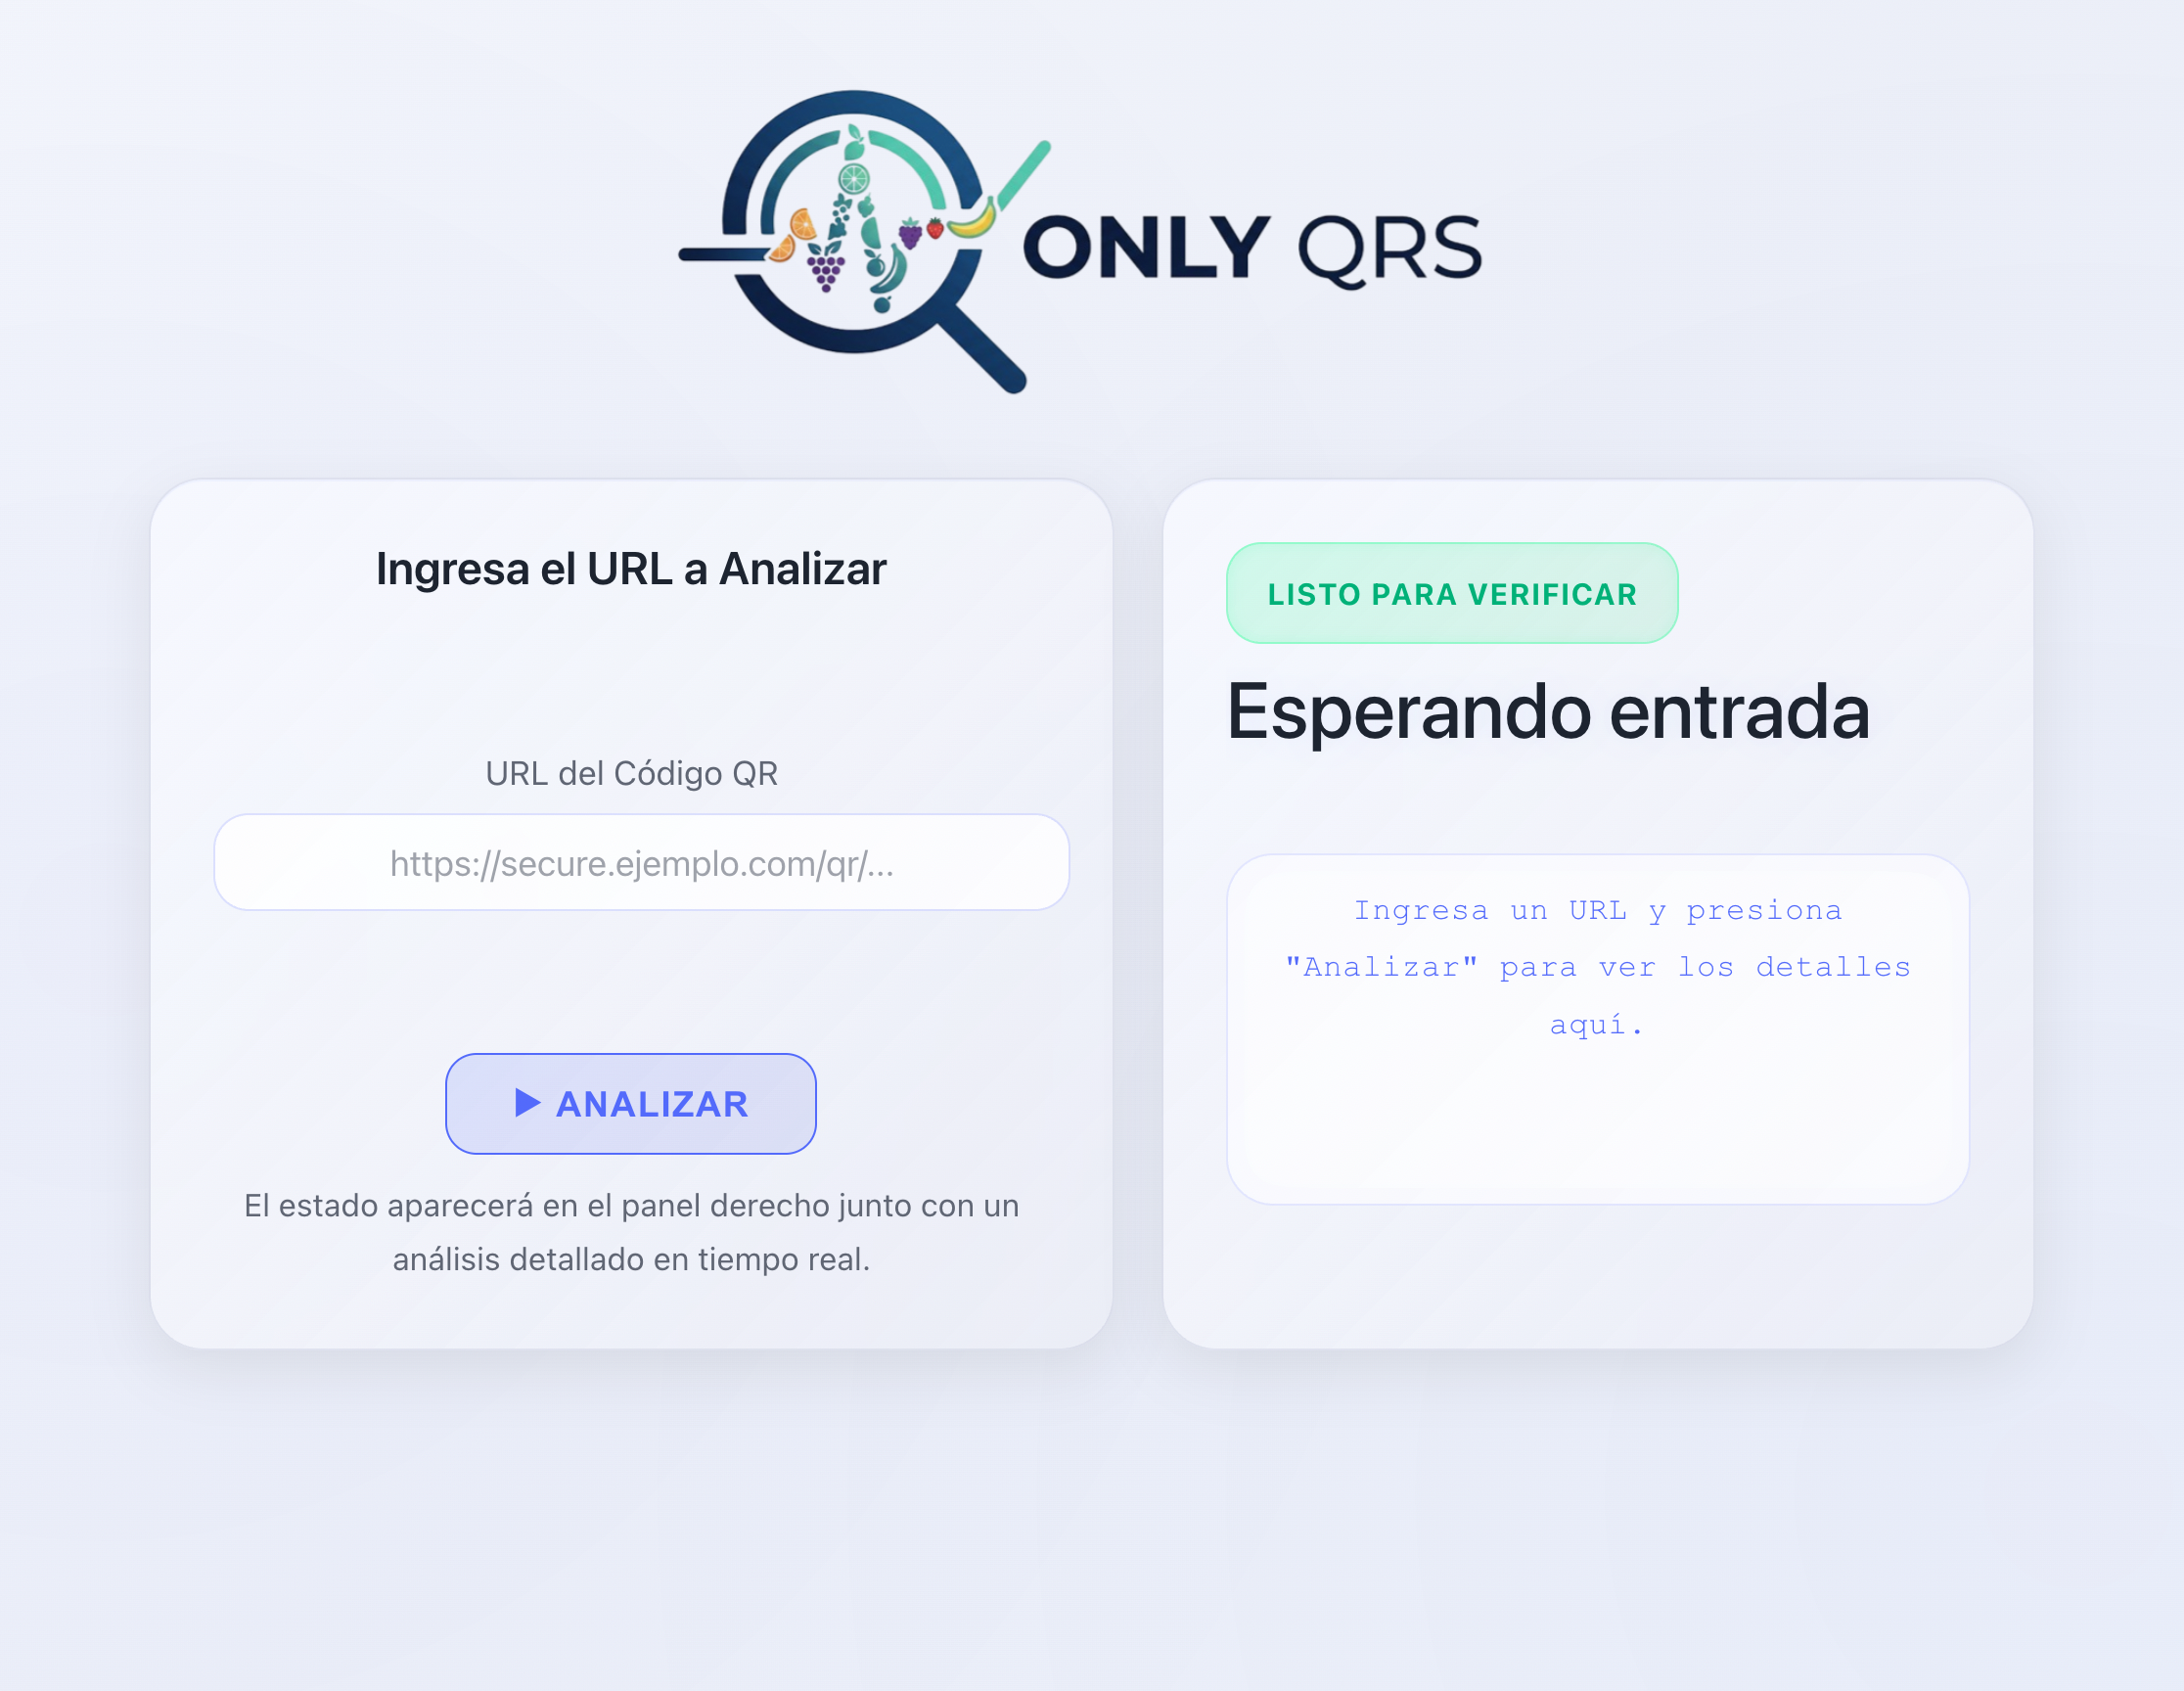
\includegraphics[
    width=\textwidth,
    height=0.75\textheight,
    keepaspectratio
]{img/ss1.png}

\end{frame}

%------------------------------------------------

\begin{frame}{Demostración de la Aplicación: Web}

\centering

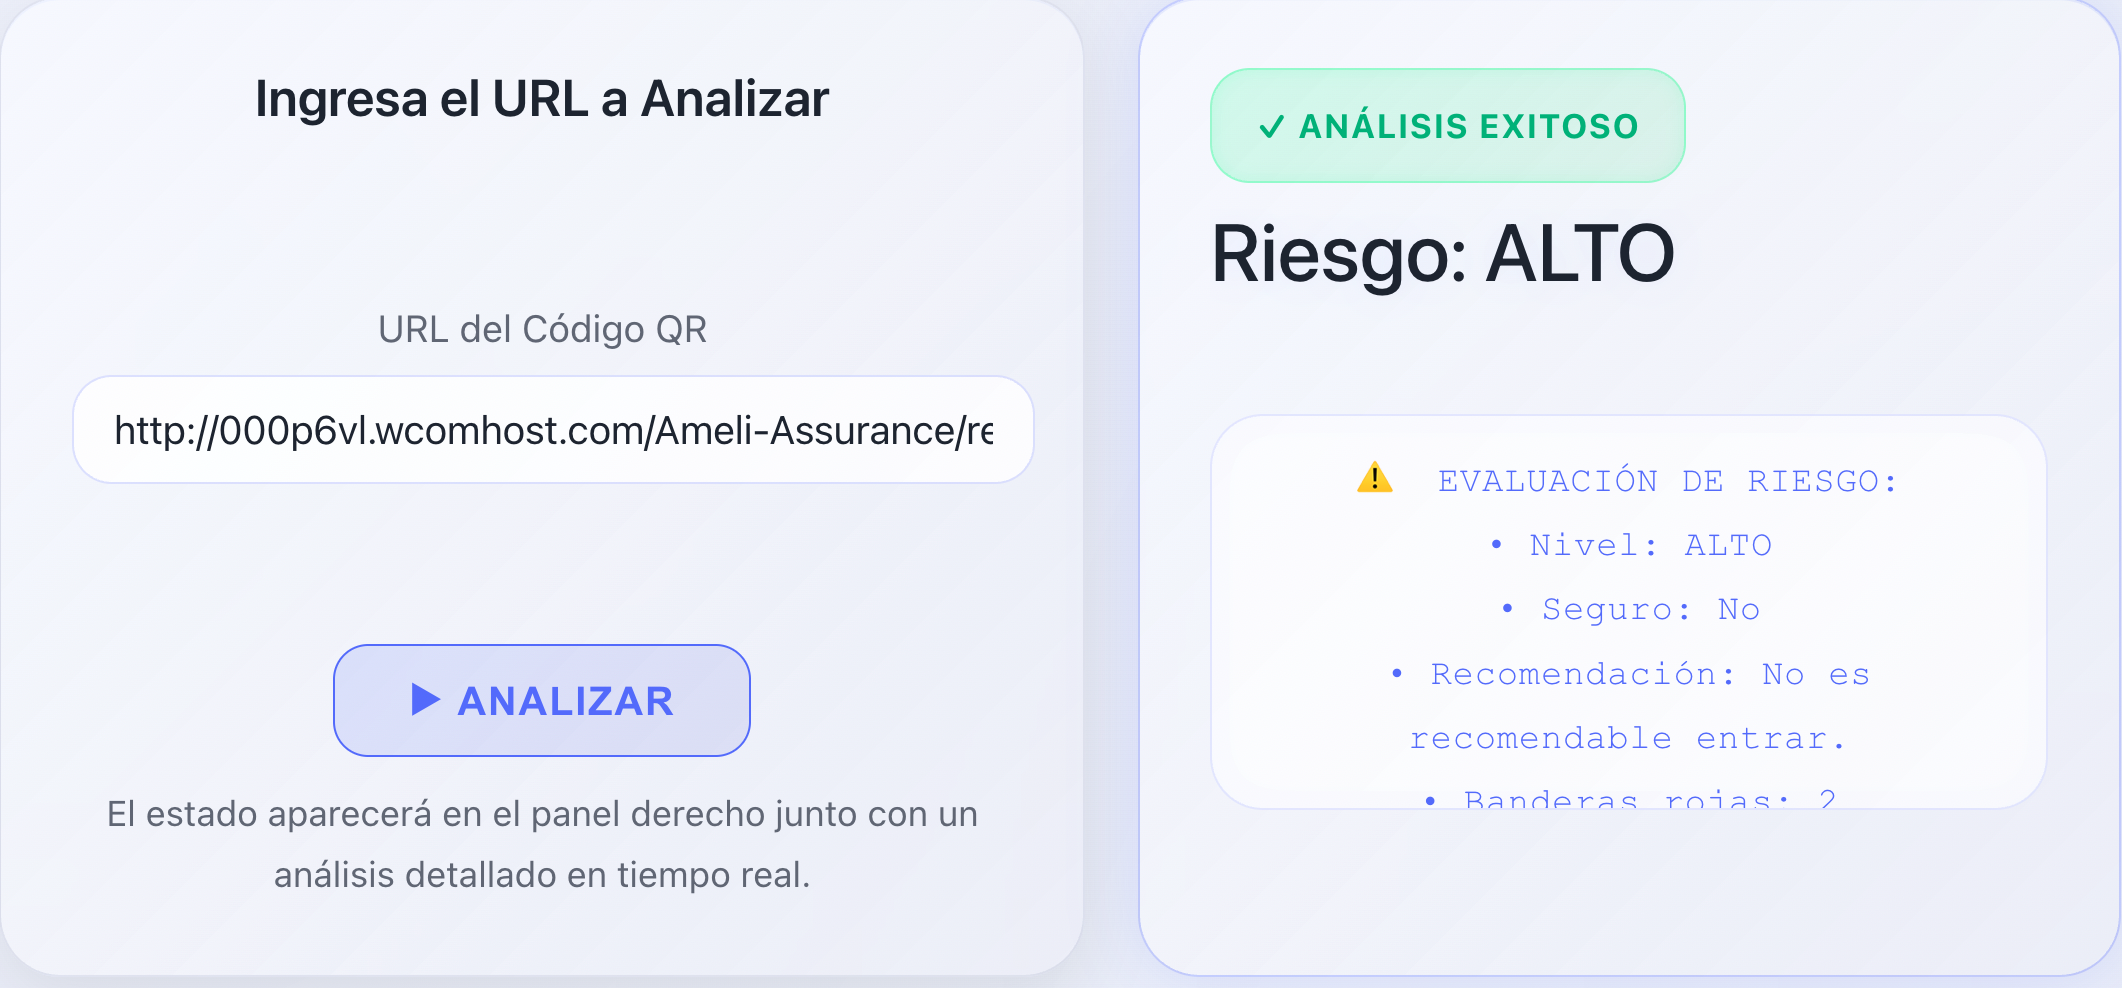
\includegraphics[
    width=\textwidth,
    height=0.75\textheight,
    keepaspectratio
]{img/ss2.png}

\end{frame}

%------------------------------------------------
\begin{frame}{Resultados Obtenidos}

\begin{itemize}
    \item URLs legítimas clasificadas correctamente.
    \item URLs maliciosas detectadas mediante VirusTotal.
    \item Integración estable durante las pruebas.
    \item Validación técnica exitosa del sistema.
\end{itemize}

\vspace{0.5cm}

\textbf{Limitación:}
\begin{itemize}
    \item No se realizaron pruebas con usuarios externos.
\end{itemize}

\end{frame}

%------------------------------------------------

\begin{frame}{Aprendizajes y Trabajo Futuro}

\textbf{Aprendizajes}

\begin{itemize}
    \item La detección de amenazas es más compleja de lo esperado.
    \item Mantener inteligencia de amenazas actualizada es difícil.
    \item VirusTotal aporta múltiples motores de detección.
\end{itemize}

\vspace{0.5cm}

\textbf{Trabajo Futuro}

\begin{itemize}
    \item Aplicación móvil.
    \item Integración directa con la cámara.
    \item Análisis automático de QRs en tiempo real.
\end{itemize}

\end{frame}

%------------------------------------------------

\begin{frame}
\centering

\Huge ¡Gracias!

\vspace{0.5cm}

\Large Preguntas

\end{frame}

%------------------------------------------------

\end{document}